\documentclass[tikz,border=2pt]{standalone}
\usepackage{amsmath,amssymb}
\usepackage{tikz}
\usetikzlibrary{arrows.meta}

\begin{document}
% Maximise f subject to g(x) <= b: the feasible region lies below the line, the unconstrained
% maximum is infeasible, and at the constrained maximum the gradient of f points OUT of the
% feasible side, as a nonnegative multiple of the constraint gradient.
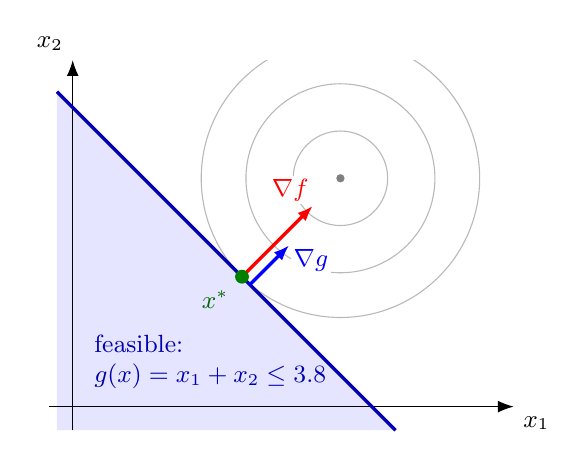
\begin{tikzpicture}[every node/.style={font=\small}, >={Latex[length=2mm]}, lab/.style={font=\small, fill=white, inner sep=1pt}]
	\fill[blue!10] (-0.2,-0.3) -- (4.1,-0.3) -- (-0.2,4.0) -- cycle;
	\begin{scope}
		\clip (-0.2,-0.3) rectangle (5.4,4.4);
		\foreach \r in {0.6,1.2,1.768} {\draw[gray!55] (3.4,2.9) circle (\r);}
	\end{scope}
	\fill[gray] (3.4,2.9) circle (1.5pt);
	\draw[->] (-0.3,0) -- (5.6,0) node[below right] {$x_1$};
	\draw[->] (0,-0.3) -- (0,4.4) node[above left] {$x_2$};
	\draw[blue!70!black, very thick] (4.1,-0.3) -- (-0.2,4.0);
	\node[blue!70!black, anchor=south west, font=\small, align=left] at (0.15,0.1) {feasible:\\ $g(x)=x_1+x_2\le3.8$};
	\draw[->, red, very thick] (2.15,1.65) -- (3.05,2.55) node[above left, lab] {$\nabla f$};
	\draw[->, blue, very thick] (2.25,1.55) -- (2.75,2.05) node[below right, lab] {$\nabla g$};
	\fill[green!50!black] (2.15,1.65) circle (2.5pt);
	\node[green!40!black, anchor=north east, font=\small] at (2.1,1.6) {$x^\ast$};
\end{tikzpicture}
\end{document}
